\documentclass[12pt,a4paper,titlepage]{article}
\usepackage[utf8]{inputenc}
\usepackage[spanish]{babel}
\usepackage[T1]{fontenc}
\usepackage[pdftex]{color,graphicx}
\usepackage{listings}
\usepackage{url}

\definecolor{gray}{RGB}{127,127,127}
\newcommand{\HRule}{\rule{\linewidth}{0.5mm}}

\lstset{
language=Java,                          	% Code langugage
basicstyle=\ttfamily,                   	% Code font
numbers=left,                           	% Line nums position
numberstyle=\tiny,                      	% Line-numbers fonts
stepnumber=1,                           	% Step between two line-numbers
numbersep=5pt,                          	% How far are line-numbers from code
frame=none,                             	% A frame around the code
tabsize=4,                              	% Default tab size
captionpos=b,                           	% Caption-position = bottom
breaklines=true,                        	% Automatic line breaking?
breakatwhitespace=false,                	% Automatic breaks only at whitespace?
showspaces=false,                       	% Dont make spaces visible
showtabs=false,                         	% Dont make tabls visible
linewidth=\textwidth,                   	% Defines the base line width
commentstyle=\color{gray}
}

\author{
	Daniel Garabato Míguez
	\and Vanesa López Beade
	\and Daniel Valcarce Silva
}
\title{Memoria Práctica LN}
\date{Curso 2012-2013}

\begin{document}

% Título
\begin{titlepage}
\begin{center}

\includegraphics[width=10cm]{res/logo_udc}\\
\vspace{1cm}
\textsc{\Large Lenguajes Naturales}\\[0.5cm]
\textsc{\Large Curso 2012/2013}\\[0.5cm]

\HRule \\[0.4cm]
{ \huge \bfseries My Little Trivial Player}\\[0.4cm]
{ \Large \bfseries Memoria de la Práctica}\\[0cm]

\HRule \\[0cm]
\end{center}

\vfill
\emph{Autores:}
\vspace{0.5cm}
\\
\vspace{0.1cm}
Garabato Míguez, Daniel \texttt{<daniel.garabato@udc.es>}\\
\vspace{0.1cm}
López Beade, Vanesa \texttt{<vanesa.lopezb@udc.es>}\\
\vspace{0.1cm}
Valcarce Silva, Daniel \texttt{<daniel.valcarce@udc.es>} (Portavoz)\\

\end{titlepage}


% Índice
\tableofcontents
\clearpage

%Cuerpo
\section{Introducción}
El objetivo de la presente práctica es realizar la implementación de un sistema de búsqueda de respuestas (\emph{question answering}). Para ello, en primer lugar, diseñaremos una arquitectura general del sistema. A continuación, se especificará el funcionamiento de cada uno de los módulos y como se implementará.

Consideraremos diferentes estrategias a la hora de resolver los diferentes problemas y las evaluaremos para quedarnos con las que nos den mejores resultados.

\section{Arquitectura del sistema}
Basándonos en varios modelos conceptuales de un sistema de búsqueda de respuestas (\cite{modelo1}, \cite{modelo2}) y el dado en la asignatura, hemos desarrollado nuestra propia arquitectura que puede verse en la Figura \ref{fig:arquitectura}.

\begin{figure}[h!]
\begin{center}
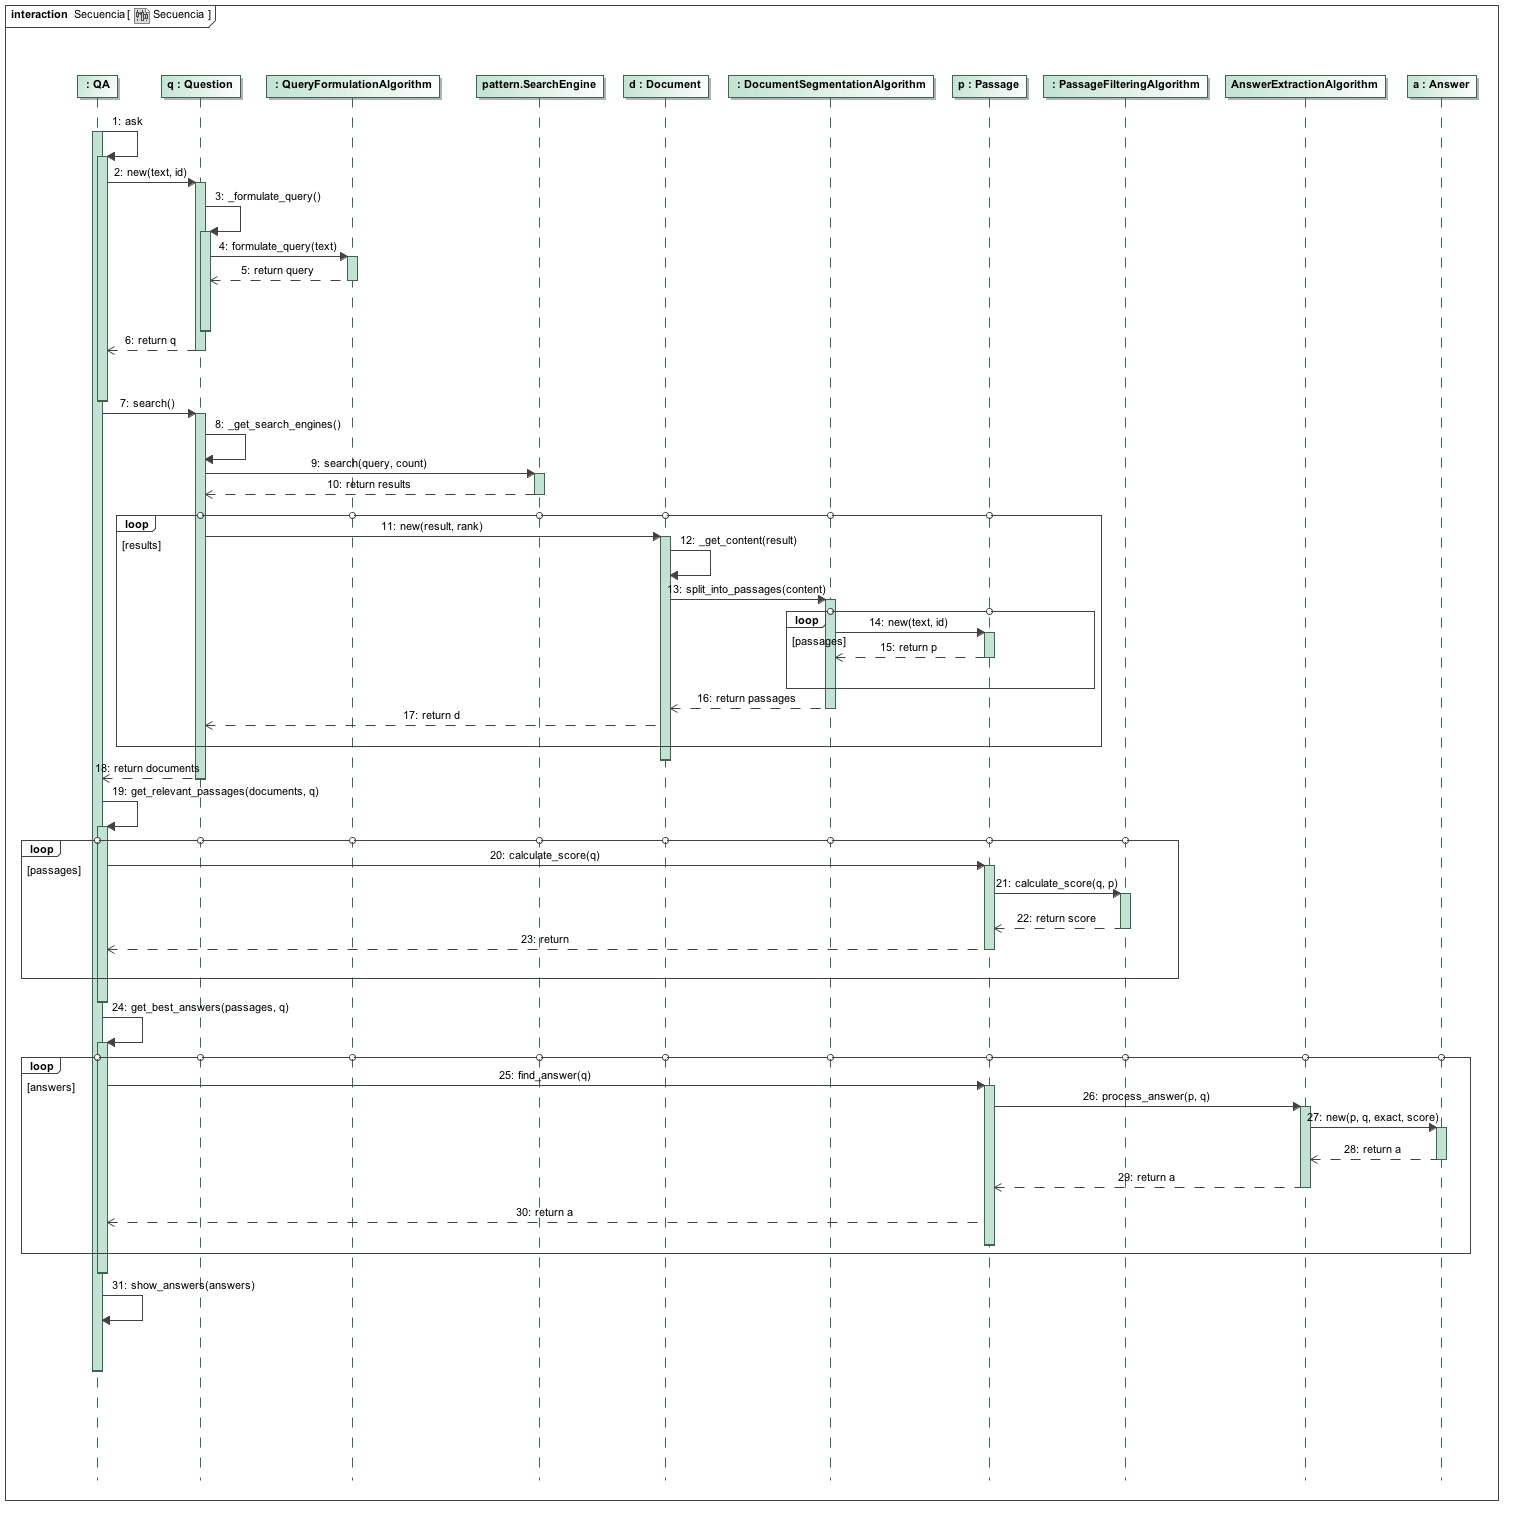
\includegraphics[width=\textwidth]{res/secuencia}
\end{center}
\caption{Arquitectura general del sistema}
\label{fig:arquitectura}
\end{figure}

\begin{description}
	\item[Query Formulation] A partir de una pregunta en lenguaje natural genera una consulta (\emph{query}) que será posteriormente interpretada por un motor de búsqueda web.
	\item[Document Retrieval] Obtiene una lista de documentos tras realizar la consulta pertinente en los motores de búsqueda. 
	\item[Passage Retrieval] Devuelve los pasajes relevantes de la lista de documentos anterior.
		\begin{description}
			\item[Document Segmentation] Divide cada documento en pasajes.
			\item[Passage Filtering] Selecciona los pasajes más relevantes.
		\end{description}
	\item[Answer Procesing] Genera las respuestas asociadas a los pasajes relevantes.
		\begin{description}
			\item[Answer Extraction] Extrae las respuestas asociadas a cada pasaje.
			\item[Answer Filtering]	Filtra las mejores respuestas.
		\end{description}
\end{description}

\subsection{Proceso de búsqueda}
Para ilustrar el proceso de búsqueda de respuestas del sistema, hemos elaborado un diagrama de secuencia que puede verse en la Figura \ref{fig:secuencia}.

\begin{figure}[h!]
\begin{center}
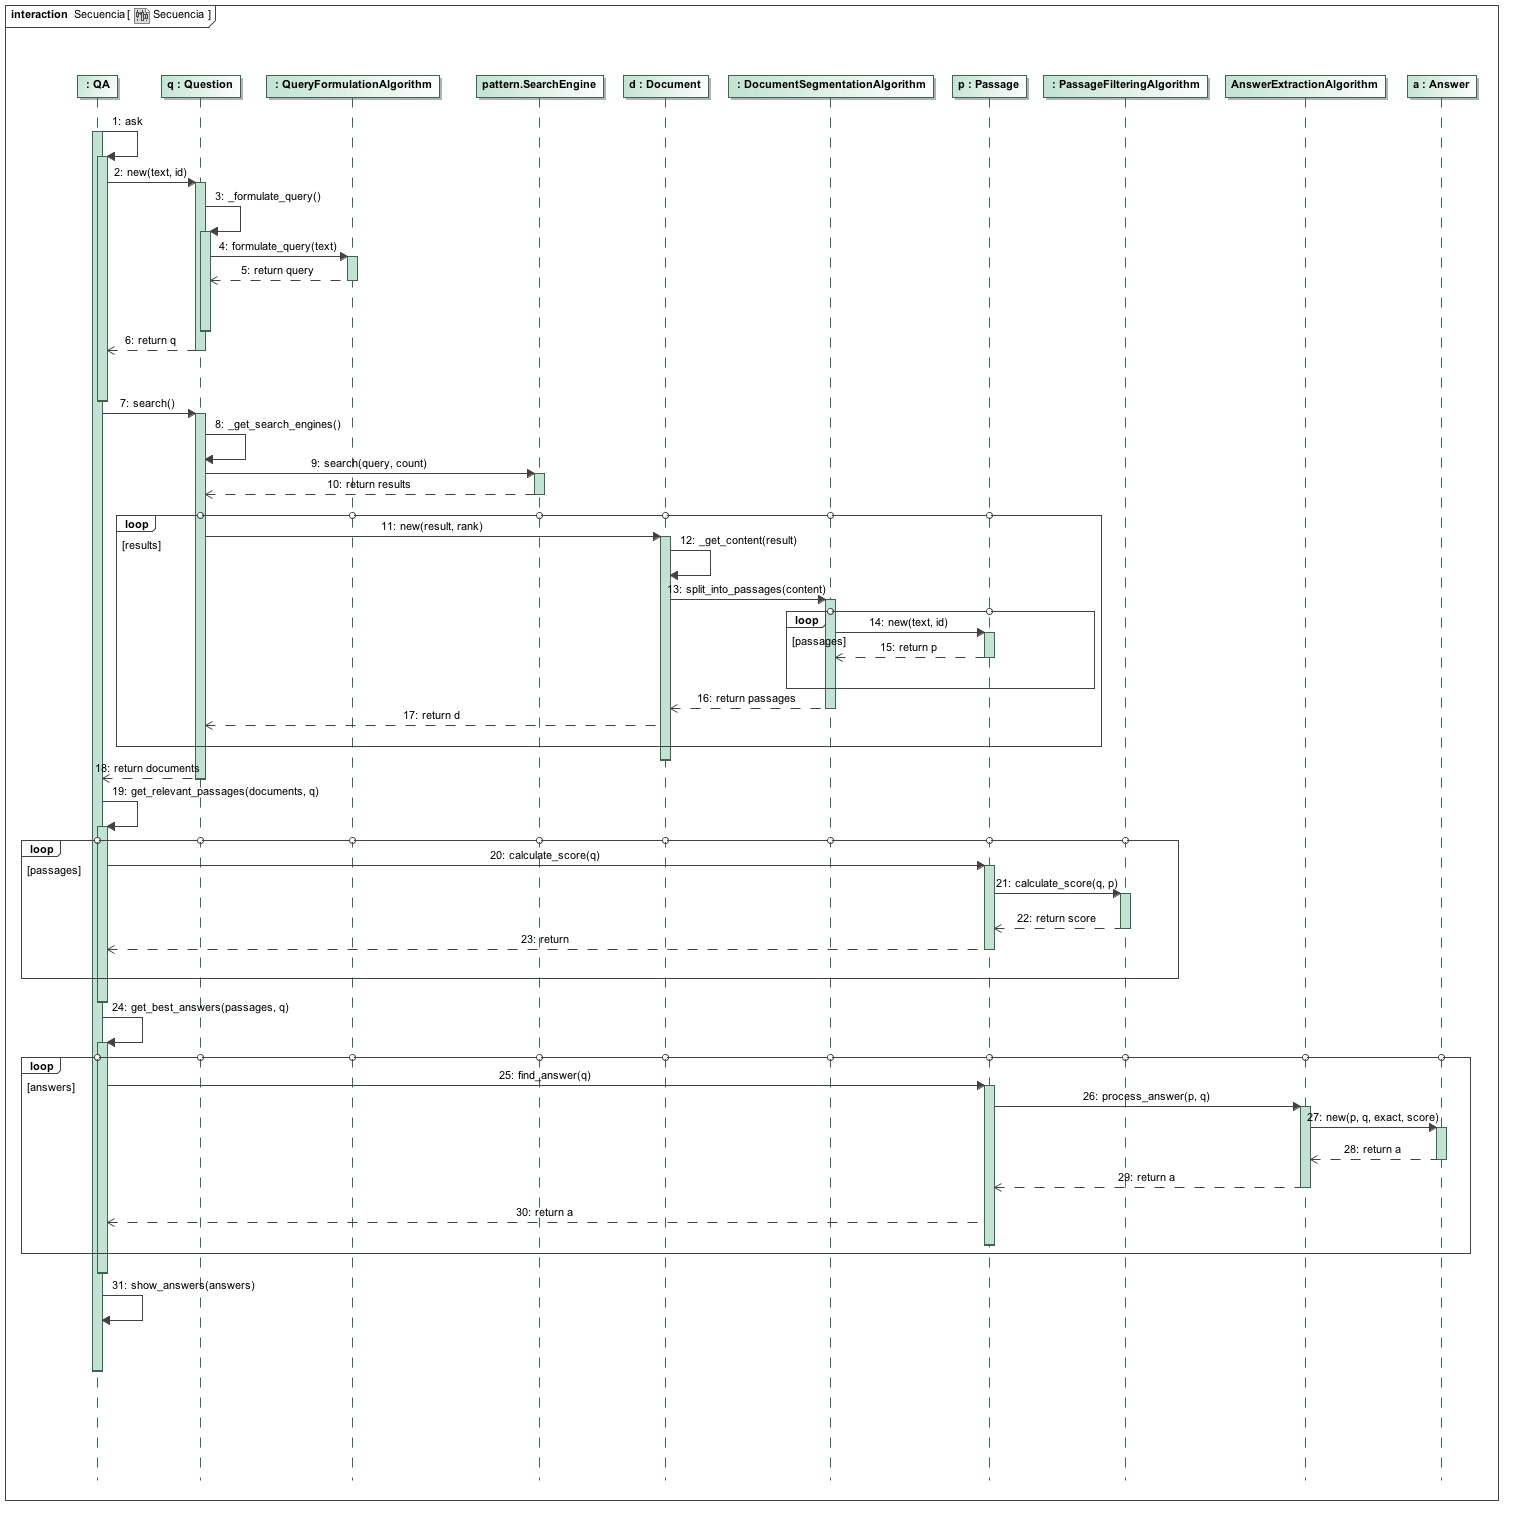
\includegraphics[width=\textwidth]{res/secuencia}
\end{center}
\caption{Diagrama de secuencia del proceso de búsqueda de respuestas}
\label{fig:secuencia}
\end{figure}

\clearpage
\section{Herramientas empleadas}


\begin{description}
	\item[NLTK] Framework libre de procesamiento de lenguaje natural para Python. Puede descargarse en \cite{nltk}.
	\item[Pattern] Módulo de \emph{web mining} libre para Python. Puede descargarse en \cite{pattern}.
	\item[PDFMiner] Módulo de Python para la extracción de información de docuemntos PDF. Más información en \cite{pdfminer}.
	\item[Git] Sistema de control de versiones distribuido libre. Puede descargarse en \cite{git}.
	\item[BitBucket] Repositorio online para git. Puede accederse a él en \cite{bitbucket}.
	\item[\LaTeX] Sistema de composición de textos con el que se ha elborado el presente documento. Más información en \cite{latex}.
	
\end{description}


\clearpage
\section{Manual de instalación y uso}

\subsection{Instalación del sistema}

\subsubsection{NLTK}
sudo pip install -U nltk
nltk.download()

\subsubsection{Google API}

sudo pip install -u pdfminer

\subsubsection{Bing API}



\subsection{Uso del sistema}



\clearpage
\section{Algoritmos}
\subsection{Query Formulation}
\subsubsection{Stopwords}

\subsection{Document Segmentation}
\subsubsection{Fixed Number off Lines}
\subsubsection{Split into Paragraphs}

\subsection{Passage Filtering}
\subsubsection{Similarity}

\subsection{Answer Extraction}
\subsubsection{Entity Recognition}
\label{s:ne_recog}

\clearpage
\section{Diario de trabajo}
A continuación se muestra un resumen del trabajo realizado a lo largo de la elaboración de la presente práctica. Las entradas se ordenan por su fecha cronológica y describen brevemente las decisiones y las acciones tomadas.


\subsubsection*{2012/10/26}
En la primera reunión del grupo, hemos discutido sobre los primeros pasos a la hora de enfrentar la práctica. Tras un análisis de los diferentes \emph{toolkits} que se nos presentan en el enunciado de la práctica, nos decidimos a usar NLTK por dos razones principales. El primer motivo es la gran cantidad de módulos que posee y su amplia documentación. En segundo lugar, porque Python nos parece un lenguaje muy cómodo para el desarrollo del proyecto.

Profundizando más en el desarrollo del trabajo, decidimos usar Git como sistema de control de versiones y apoyarnos en un repositorio privado de Bitbucket. Esto nos permitirá tener nuestro código bien organizado y documentado así como proporcionarnos un respaldo de los datos.

Por último, acordamos documentarnos más sobre el uso de Python en el procesamiento de lenguaje natural en general y con NLTK en particular. Para ello recurriremos a la bibliografía recomendada por los creadores del toolkit \cite{nltk-book}. También optamos por estudiar las APIs de Google y de Bing para realizar consultas.

\subsubsection*{2012/10/29}
Hemos instalado y configurado NLTK. Hemos estudiado utilizar el módulo Pattern (en Python) para la implementación de las consultas en los buscadores (Google y Bing). Hemos solicitado unas claves para poder utilizar las APIs de dichos buscadores.

Por otro lado, hemos comenzado a estudiar la formulación de la consulta (\emph{query formulation}). Debemos eliminar aquellas palabras innecesarias (\emph{stopwords}) por lo que utilizamos el diccionario de Porter ya integrado en NLTK. Consideramos mantener las comillas y los apóstrofes ya que dan mejores resultados en los buscadores. Optamos por no eliminar la interrogación final puesto que es irrelevante para ellos.

\subsubsection*{2012/11/05}
Se ha dedicado la tarde del presente día a la implementación de la búsqueda de información en los buscadores web (a saber, Google y Bing). Hemos comenzado empleando la biblioteca Pattern\cite{pattern-web} la cual nos aporta una interfaz adaptador entre el API de los buscadores y nuestro sistema. No obstante, tras las pruebas iniciales comprobamos que el servidor de Google devolvía un error HTTP400 Bad Request a nuestras peticiones.

Al no encontrar solución a este problema, dedujimos que sería un bug en la biblioteca Pattern por lo que comenzamos a desarrollar nuestra propia biblioteca para integrar las APIs de los buscadores. Tras la integración del API de Google, verificamos en las pruebas que se producía el mismo error. Buscando posibles soluciones en la web, averiguamos que el origen del error 400 no era una petición HTTP mal formada si no un error de autenticación: la clave del API que estábamos utilizando era incorrecta.

Comprobamos que efectivamente ese era el error y decidimos volver a utilizar la biblioteca Pattern en vez de seguir implementando la nuestra porque esta ya nos proporciona una acceso unificado a la información de los buscadores.

\subsubsection*{2012/11/06}
Se ha realizado la planificación de la arquitectura del sistema de búsqueda de respuetas con el objetivo de orientar el desarrollo de los componentes que faltan. Hemos concluido crear las clases \texttt{QA}, \texttt{Query}, \texttt{Document}, \texttt{Passage} y \texttt{Answer} tras un esbozo del diagrama de clases que se ha construido a partir de un estudio de los casos de uso.

\subsubsection*{2012/11/12}
Durante la sesión de hoy hemos continuado refinando nuestro sistema realizando una adaptación de las funcionalidades ya implementadas a la arquitectura del sistema esbozada en la sesión previa.

Además se ha implementado una sencilla interfaz para la realización de las consultas. Por un lado, se ofrece la posibilidad de introducir una única consulta manualmente en el sistema y, por otro lado, permitiremos el uso de un fichero externo para realizar múltiples consultas mediante el paso de un fichero como parámetro en nuestro programa principal. El tratamiento de dicho fichero de preguntas se realiza mediante una expresión regular con el fin de proporcionar mayor robustez al sistema.

En último lugar desarrollamos la lógica necesaria para gestionar un fichero de configuración.

\subsubsection*{2012/11/13}
En primer lugar, hemos decidido crear una clase \texttt{MyConfig} cuyo objetivo es encapsular la forma de acceder al fichero de configuración.

A continuación hemos utilizado el módulo pickle de Python para serializar los documentos resultantes de realizar la consulta en los buscadores.

Por último, se ha desarrollado código capaz de manejar distintos tipos de documentos que nos podemos encontrar por la red:
\begin{itemize}
\item Los ficheros HTML se tratan con un procesador dedicado a ello que elimina las etiquetas, el código CSS o JavaScript, etc.
\item Los archivos en texto plano no necesitan procesamiento.
\item Aquellos documentos cuyo formato no reconocemos\footnote{En un inicio pensamos en tratar de forma especial documentos ofimáticos (.doc, .docx, .xls, .xlsx, .ppt, .pptx, OpenDocument...); sin embargo, la probabilidad de encontrárselos como resultado de la búsqueda generada por una pregunta factual es muy baja y el tratamiento genérico que hemos implementado da unos resultados satisfactorios.} son manejados de una forma genérica: mediante una expresión regular extraemos los caracteres legibles de los mismos.
\end{itemize}

\subsubsection*{2012/11/19}
Hemos comenzado con la división de los documentos en pasajes. Consideramos oportuno que los fragmentos sean solapados para evitar la posible pérdida de información. En principio hemos decidido segmentar los documentos por líneas ---el número de ellas será especificado en el fichero de configuración---.

Posteriormente, se ha implementado el uso de logs mediante el módulo logging de Python. Hemos creado un fichero de configuración para tal efecto.

\subsubsection*{2012/11/20}
En primer lugar, hemos reestructurado el proyecto para utilizar el patrón estrategia para los algoritmos de formulación de consultas, puntuación de pasajes y procesamiento de respuestas.

Hemos desarrollado nuestra primera heurística para la evaluación de la relevancia de los pasajes en la búsqueda de respuestas. El algoritmo se basa en la similitud entre el pasaje y la pregunta. Se limpia la pregunta y el pasaje de símbolos y stopwords. A continuación se calcula el número de palabras coincidentes. Dividimos dicha cantidad entre el número de palabras en el pasaje y lo ponderamos por la relevancia del resultado según el buscador.

Por otro lado, se ha refinado el algoritmo de formulación de consultas eliminando símbolos no deseados.

\subsubsection*{2012/11/26}
Decidimos utilizar otro patrón estrategia para la segmentación del texto en pasajes. Creamos una estrategia nueva que segmenta el texto en párrafos, complementando asi a la estrategia de segmentar por un número fijo de líneas.

Mejoramos el algoritmo de filtrado de pasajes relevantes por similitud aplicando \emph{stemming} a la pregunta y al pasaje mediante el uso del Stemmer de Porter. Probamos además el uso de un lematizador basado en WordNet, pero tras su prueba descartamos su utilización ya que discriminaba menos casos similares.

Documentamos el fichero de configuración con los posibles algoritmos a emplear (formulación de consultas, segmentación en pasajes, búsqueda de pasajes relevantes y procesamiento de respuestas).

Implementamos lógica adicional para la gestión de las respuestas y su correcta visualización de acuerdo a las normas del enunciado de la práctica.

\subsubsection*{2012/11/27}
Durante el día de hoy se ha diseñado el gráfico de arquitectura del sistema, estableciendo los diferentes módulos que componen el mismo:

\begin{itemize}
\item Query Formulation 
\item Document Retrieval
\item Passage Retrieval
	\begin{itemize}
	\item Document Segmentation
	\item Passage Filtering 
	\end{itemize}
\item Answer Processing
	\begin{itemize}
	\item Answer Extraction
	\item Answer Filtering
	\end{itemize}
\end{itemize}

Así mismo hemos elaborado un diagrama de secuencia en el que se expone el funcionamiento global del sistema (puesto que éste solo contempla un único caso de uso: realizar consultas).

\subsubsection*{2012/12/03}
Corrección de múltiples errores en diferentes módulos de la práctica.

Hemos considerado que una consulta en diferentes motores de búsqueda nos puede dar los mismos documentos como resultado; por tanto, se ha decidido controlar la posible repetición de documentos para evitar duplicados.

\subsubsection*{2012/12/04}
Añadimos la escritura de resultados en un fichero.

Implementamos la lógica necesaria para gestionar la posible falta de respuestas. Por un lado, si los motores de búsqueda no nos devuelven resultados deolvemos NIL con la puntuación máxima. Por otro lado, si no encontramos una buena respuesta en los documentos de la web devolvemos NIL con la puntuación mínima. Por último si el número de respuestas admisibles es menor que tres, las mostramos y añadimos un NIL con puntuación mínima.

En el fichero de configuración, podemos especificar el umbral de lo que consideramos una respuesta admisible.

\subsubsection*{2012/12/10}
Creamos un algoritmo de Answer Extraction basado en la técnica de Named Entities Recognition explicado en la Sección \ref{s:ne_recog}. Queda por completar la parte de Query Classification (de momento solo admitimos preguntas sobre personas).

Mejoramos nuestra metodología de Answer Filtering ponderando las puntuaciones de las respuestas por su frecuencia relativa de aparición en los pasajes relevantes.

Realizamos las primeras pruebas sobre un sistema ya funcional y obtenemos buenos resultados ---en principio--- para preguntas relacionadas con personas. Las respuestas están motivadas correctamente y la tasa de aciertos ronda el 20\%. Consideramos esto un hito en el desarrollo del sistema ya que tenemos una primera versión preliminar que proporciona resultados coherentes.

\subsubsection*{2012/12/11}
Dedicamos el día de hoy a implementar técnicas de Question Classification. Utilizamos dos modelos: un clasificador bayesiano ingenuo y un modelo de máxima entropía proporcionados por NLTK.

Modificamos el corpus qc del NLTK para que se adapte a nuestras entidades y entrenamos ambos sistemas. Obtenemos una precisión algo más elevada en el caso del modelo de máxima entropía.

Consideramos realizar para el próximo día la integración del Named Entity Recognizer de Stanford puesto que los resultados del reconocedor de entidades del NLTK no son muy satisfactorios en algunos casos.

\subsubsection*{2012/12/17}
Hemos implementado dos técnicas para detectar números y otros tipos de entidades (NUMBER y OTHER, respectivamente). Los números se reconocen como caracteres numérico o como sustantivos y adjetivos numerales. El reconocimiento de otro tipo de entidades se realiza mediante la extración de sustantivos (exceptuando aquellos que son entidades).

Realizamos también pequeñas refactorizaciones del código. Optimizamos la técnica de Question Classification mediante el uso de una caché de preguntas.

\clearpage
\section{Bibliografía}
\begin{thebibliography}{99}

\bibitem{nltk}
NLTK: \url{http://www.nltk.org}.

\bibitem{nltk-book}
S. Bird, E. Klein, E. Loper: \emph{Natural Language Processing with Python --- Analyzing Text with the Natural Language Toolkit}, O'Reilly Media (2009).

\bibitem{pattern}
CLIPS Pattern: \url{http://www.clips.ua.ac.be/pages/pattern}.

\bibitem{pdfminer}
PDFMiner: \url{http://www.unixuser.org/~euske/python/pdfminer/index.html}.

\bibitem{git}
Git: \url{http://www.git-scm.com}.

\bibitem{bitbucket}
BitBucket: \url{http://www.bitbucket.org/daniel_garabato/ln}.

\bibitem{latex}
\LaTeX: \url{http://www.latex-project.org}.

\end{thebibliography}


\end{document}
